% Options for packages loaded elsewhere
\PassOptionsToPackage{unicode}{hyperref}
\PassOptionsToPackage{hyphens}{url}
%
\documentclass[
]{article}
\usepackage{amsmath,amssymb}
\usepackage{iftex}
\ifPDFTeX
  \usepackage[T1]{fontenc}
  \usepackage[utf8]{inputenc}
  \usepackage{textcomp} % provide euro and other symbols
\else % if luatex or xetex
  \usepackage{unicode-math} % this also loads fontspec
  \defaultfontfeatures{Scale=MatchLowercase}
  \defaultfontfeatures[\rmfamily]{Ligatures=TeX,Scale=1}
\fi
\usepackage{lmodern}
\ifPDFTeX\else
  % xetex/luatex font selection
\fi
% Use upquote if available, for straight quotes in verbatim environments
\IfFileExists{upquote.sty}{\usepackage{upquote}}{}
\IfFileExists{microtype.sty}{% use microtype if available
  \usepackage[]{microtype}
  \UseMicrotypeSet[protrusion]{basicmath} % disable protrusion for tt fonts
}{}
\makeatletter
\@ifundefined{KOMAClassName}{% if non-KOMA class
  \IfFileExists{parskip.sty}{%
    \usepackage{parskip}
  }{% else
    \setlength{\parindent}{0pt}
    \setlength{\parskip}{6pt plus 2pt minus 1pt}}
}{% if KOMA class
  \KOMAoptions{parskip=half}}
\makeatother
\usepackage{xcolor}
\usepackage[margin=1in]{geometry}
\usepackage{color}
\usepackage{fancyvrb}
\newcommand{\VerbBar}{|}
\newcommand{\VERB}{\Verb[commandchars=\\\{\}]}
\DefineVerbatimEnvironment{Highlighting}{Verbatim}{commandchars=\\\{\}}
% Add ',fontsize=\small' for more characters per line
\usepackage{framed}
\definecolor{shadecolor}{RGB}{248,248,248}
\newenvironment{Shaded}{\begin{snugshade}}{\end{snugshade}}
\newcommand{\AlertTok}[1]{\textcolor[rgb]{0.94,0.16,0.16}{#1}}
\newcommand{\AnnotationTok}[1]{\textcolor[rgb]{0.56,0.35,0.01}{\textbf{\textit{#1}}}}
\newcommand{\AttributeTok}[1]{\textcolor[rgb]{0.13,0.29,0.53}{#1}}
\newcommand{\BaseNTok}[1]{\textcolor[rgb]{0.00,0.00,0.81}{#1}}
\newcommand{\BuiltInTok}[1]{#1}
\newcommand{\CharTok}[1]{\textcolor[rgb]{0.31,0.60,0.02}{#1}}
\newcommand{\CommentTok}[1]{\textcolor[rgb]{0.56,0.35,0.01}{\textit{#1}}}
\newcommand{\CommentVarTok}[1]{\textcolor[rgb]{0.56,0.35,0.01}{\textbf{\textit{#1}}}}
\newcommand{\ConstantTok}[1]{\textcolor[rgb]{0.56,0.35,0.01}{#1}}
\newcommand{\ControlFlowTok}[1]{\textcolor[rgb]{0.13,0.29,0.53}{\textbf{#1}}}
\newcommand{\DataTypeTok}[1]{\textcolor[rgb]{0.13,0.29,0.53}{#1}}
\newcommand{\DecValTok}[1]{\textcolor[rgb]{0.00,0.00,0.81}{#1}}
\newcommand{\DocumentationTok}[1]{\textcolor[rgb]{0.56,0.35,0.01}{\textbf{\textit{#1}}}}
\newcommand{\ErrorTok}[1]{\textcolor[rgb]{0.64,0.00,0.00}{\textbf{#1}}}
\newcommand{\ExtensionTok}[1]{#1}
\newcommand{\FloatTok}[1]{\textcolor[rgb]{0.00,0.00,0.81}{#1}}
\newcommand{\FunctionTok}[1]{\textcolor[rgb]{0.13,0.29,0.53}{\textbf{#1}}}
\newcommand{\ImportTok}[1]{#1}
\newcommand{\InformationTok}[1]{\textcolor[rgb]{0.56,0.35,0.01}{\textbf{\textit{#1}}}}
\newcommand{\KeywordTok}[1]{\textcolor[rgb]{0.13,0.29,0.53}{\textbf{#1}}}
\newcommand{\NormalTok}[1]{#1}
\newcommand{\OperatorTok}[1]{\textcolor[rgb]{0.81,0.36,0.00}{\textbf{#1}}}
\newcommand{\OtherTok}[1]{\textcolor[rgb]{0.56,0.35,0.01}{#1}}
\newcommand{\PreprocessorTok}[1]{\textcolor[rgb]{0.56,0.35,0.01}{\textit{#1}}}
\newcommand{\RegionMarkerTok}[1]{#1}
\newcommand{\SpecialCharTok}[1]{\textcolor[rgb]{0.81,0.36,0.00}{\textbf{#1}}}
\newcommand{\SpecialStringTok}[1]{\textcolor[rgb]{0.31,0.60,0.02}{#1}}
\newcommand{\StringTok}[1]{\textcolor[rgb]{0.31,0.60,0.02}{#1}}
\newcommand{\VariableTok}[1]{\textcolor[rgb]{0.00,0.00,0.00}{#1}}
\newcommand{\VerbatimStringTok}[1]{\textcolor[rgb]{0.31,0.60,0.02}{#1}}
\newcommand{\WarningTok}[1]{\textcolor[rgb]{0.56,0.35,0.01}{\textbf{\textit{#1}}}}
\usepackage{longtable,booktabs,array}
\usepackage{calc} % for calculating minipage widths
% Correct order of tables after \paragraph or \subparagraph
\usepackage{etoolbox}
\makeatletter
\patchcmd\longtable{\par}{\if@noskipsec\mbox{}\fi\par}{}{}
\makeatother
% Allow footnotes in longtable head/foot
\IfFileExists{footnotehyper.sty}{\usepackage{footnotehyper}}{\usepackage{footnote}}
\makesavenoteenv{longtable}
\usepackage{graphicx}
\makeatletter
\def\maxwidth{\ifdim\Gin@nat@width>\linewidth\linewidth\else\Gin@nat@width\fi}
\def\maxheight{\ifdim\Gin@nat@height>\textheight\textheight\else\Gin@nat@height\fi}
\makeatother
% Scale images if necessary, so that they will not overflow the page
% margins by default, and it is still possible to overwrite the defaults
% using explicit options in \includegraphics[width, height, ...]{}
\setkeys{Gin}{width=\maxwidth,height=\maxheight,keepaspectratio}
% Set default figure placement to htbp
\makeatletter
\def\fps@figure{htbp}
\makeatother
\setlength{\emergencystretch}{3em} % prevent overfull lines
\providecommand{\tightlist}{%
  \setlength{\itemsep}{0pt}\setlength{\parskip}{0pt}}
\setcounter{secnumdepth}{-\maxdimen} % remove section numbering
\ifLuaTeX
  \usepackage{selnolig}  % disable illegal ligatures
\fi
\IfFileExists{bookmark.sty}{\usepackage{bookmark}}{\usepackage{hyperref}}
\IfFileExists{xurl.sty}{\usepackage{xurl}}{} % add URL line breaks if available
\urlstyle{same}
\hypersetup{
  pdftitle={Reproduction Analysis of Malcomb et al 2014},
  pdfauthor={Joseph Holler, Kufre Udoh, Drew An-Pham, Middlebury Open GIScience Classes},
  hidelinks,
  pdfcreator={LaTeX via pandoc}}

\title{Reproduction Analysis of Malcomb et al 2014}
\author{Joseph Holler, Kufre Udoh, Drew An-Pham, Middlebury Open
GIScience Classes}
\date{2023-10-21}

\begin{document}
\maketitle

\hypertarget{abstract}{%
\section{Abstract}\label{abstract}}

Malcomb, Weaver and Krakowka
(\href{https://doi.org/10.1016/j.apgeog.2014.01.004}{2014}) published
one of the first sub-national geographic climate change vulnerability
models for a developing country (1.4). The authors intended for the
study to be replicable across space (other African countries with
similar data available) (7.1), time (when new survey data is published)
(4.5 and 7.1), and vulnerability stimuli (7.1). The study's social
impacts are to address extreme vulnerability to climate change (1.3) and
assisting in the allocation and evaluation of foreign aid (1.2). The
methodology was designed to be ``transparent and easily replicable''
(2.1) in its use of ``locally derived indicators and granular data''
(2.1). The study was designed to address critiques of vulnerability
models aimed at their uncertainty and sensitivity due to problems of
scale and spatial aggregation, normative and subjective modelling
decisions, and data availability, and challenges in model comparability
(2.1). The model uses household adaptive capacity data from the United
States Agency for International Development (USAID) Demographic and
Health Surveys (DHS) (1.4 and 4.1) available in 44 African countries
(7.1), livelihood sensitivity data from the USAID / Famine Early Warning
Systems Network (FEWSnet) livelihood zones baseline surveys available in
23 African countries (3.6), and global physical exposure data from the
United Nations Environment Programme (UNEP) Global Risk Data Platform.

This replication study is motivated by three factors. First, there is an
urgent need to evaluate the reproducibility of research in
human-environment and geographical sciences (HEGS) and to establish
protocols and infrastructure for conducting and publishing
reproduction/replication studies and reproducible research in HEGS.
Second, a fully reproducible publication can be more readily replicated
in new geographic, temporal, and thematic contexts, and tested for
uncertainty due to data constraints and subjective modelling decisions.
Third, climate change is causing increasingly severe in Africa.
Improving the reproducibility and replicability of climate vulnerability
research will hopefully enhance the potential for research to inform
policy and reduce harm caused by climate change.

Malcomb et al (2014) produce two models of interest for Malawi. Figure
4, labelled ``Malawi Household Resilience'', visualizes the average
adaptive capacity score of households in each traditional authority.
Figure 5, labelled ``Malawi Composite Vulnerability Index'', visualizes
vulnerability scores by locations (cells) in a continuous raster grid.
In this study, we will attempt to identically reproduce figure 4
(adaptive capacity by traditional authority) and figure 5 (vulnerability
grid) using The R Project for Statistical Computing and the same data
sources cited in the original publication. We will visually compare our
resulting reproduction figures with the original figures. Comparison
will be aided by digitizing and joining the original figure results to
the reproduction results for each model, and then calculating any
differences between them. Differences will be visualized with thematic
maps for both models, a confusion matrix for figure 4 (adaptive capacity
by traditional authority), and a scatterplot for figure 5 (vulnerability
grid). An exact reproduction should produce exact replicas of the rank
order of traditional authorities by adaptive capacity and grid cells by
vulnerability. We will test this with the Spearman's Rho Correlation
Coefficient, expecting values of 1 for perfect correlation.

The original study is a descriptive geographic multi-criteria analysis
based on local expert opinion, and therefore has no testable hypotheses
or effects.

The replication study data and code will be made available in a GitHub
repository to the greatest extent that licensing and file sizes permit.
The repository will be made public at
\href{https://github.com/HEGSRR/RPr-Malcomb-2014}{github.com/HEGSRR/RPr-Malcomb-2014}

Malcomb, D. W., E. A. Weaver, and A. R. Krakowka. 2014. Vulnerability
modeling for sub-Saharan Africa: An operationalized approach in Malawi.
\emph{Applied Geography} 48:17--30.
\url{DOI:\%5B10.1016/j.apgeog.2014.01.004}{]}(\url{https://doi.org/10.1016/j.apgeog.2014.01.004}).

\hypertarget{keywords}{%
\subsubsection{Keywords}\label{keywords}}

Reproducibility, Vulnerability, GIS, Climate Change, Africa

\hypertarget{study-design}{%
\subsection{Study design}\label{study-design}}

The reproduction study design will first implement the original study as
closely as possible to reproduce the 2010 Household Resilience map (F4)
and Malawi Vulnerability Map (F5). Our two confirmatory hypotheses are
that we will be able to independently reproduce results for both maps.

The working hypotheses are therefore:

\begin{quote}
H1: There is no perfect positive correlation between Malcomb et al's
ranking of traditional authorities by household resilience and our
reproduction study's ranking of traditional authorities by household
resilience.
\end{quote}

\begin{quote}
H2: There is no perfect positive between Malcom et al's ranking of
locations by climate vulnerability and our reproduction study's ranking
of locations by climate vulnerability.
\end{quote}

We will evaluate each of these hypotheses using a Spearman's Rho
Correlation. A failure to reject these hypotheses would indicate that
our results do not exactly match those of the original authors. A
positive correlation approaching 1 would indicate a partial reproduction

\hypertarget{original-study-design}{%
\subsubsection{Original study design}\label{original-study-design}}

The original study is \textbf{observational} and \textbf{descriptive},
with no hypotheses or effect sizes. The study is a multi-criteria
analysis using geographic information systems (GIS) to implement a
hierarchical geographic model of climate change vulnerability model in
Malawi.

The \textbf{spatial extent} of the study was the country of Malawi. The
\textbf{spatial scale} of the study was the third administrative level
(traditional authorities) and a raster grid of unknown spatial
resolution. The \textbf{temporal extent} of the study was explicitly
2004---2010 (4.5), but the contains secondary data collected earlier
(3.6 and F5).

The model themes, indicators, and weights were selected based upon 70
interviews and 11 village focus groups from field trips to Malawi in
March and August of 2011 (1.4, 4.2 and A1). Themes and indicators were
also contextualized in literature (3.3 through 3.7) and adjusted based
on redundancy and representativeness across the country (4.3). The model
and weights were adjusted through ``several iterations of the model
using alternative weighting schemes'' (4.3) to produce a ``final product
that reflects Malawi's contextual and perceptual vulnerability'' (4.3).
Each theme was constructed of indicators from a single data provider:
adaptive capacity is measured with USAID DHS surveys, livelihood
sensitivity is measured with FEWSnet/Malawi Vulnerability Assessment
Committee (MVAC) livelihood zones baseline data, and physical exposure
is measured with UNEP Global Risk Data Platform data (T1 and T2).
Although the authors emphasize a grounded local evidence-based selection
of indicators and weights (2.1, 4.2, 5.1 and 7.1), other evidence in the
publication suggests a model design based on a more pragmatic
combination of factors including expert local opinion, deductive theory,
and the availability and characteristics of data.

The study did not use any \textbf{randomization}.

The original study was conducted using STATA™ (4.4) and ArcGIS™ (4.6, F3
and F4) with unspecified software versions, by 2012 according to
creation dates on map figures (F3, F4 and F5).

\hypertarget{computational-environment}{%
\section{Computational environment}\label{computational-environment}}

The study was originally conducted using ArcGIS and unspecified
statistical software. This reproduction study uses R, including the rdhs
package for DHS survey data, the sf package for vector analysis, the
stars package for raster analysis, and the tmap package for cartography.

\begin{Shaded}
\begin{Highlighting}[]
\CommentTok{\# set up default knitr parameters}
\NormalTok{knitr}\SpecialCharTok{::}\NormalTok{opts\_chunk}\SpecialCharTok{$}\FunctionTok{set}\NormalTok{(}
  \AttributeTok{echo =} \ConstantTok{FALSE}\NormalTok{,}
  \AttributeTok{fig.width =} \DecValTok{8}\NormalTok{,}
  \AttributeTok{fig.path =} \FunctionTok{paste0}\NormalTok{(}\FunctionTok{here}\NormalTok{(}\StringTok{"results"}\NormalTok{, }\StringTok{"figures"}\NormalTok{), }\StringTok{"/"}\NormalTok{)}
\NormalTok{)}

\CommentTok{\# these values allow you to access private and public raw data more efficiently}
\NormalTok{private\_r }\OtherTok{\textless{}{-}} \FunctionTok{here}\NormalTok{(}\StringTok{"data"}\NormalTok{, }\StringTok{"raw"}\NormalTok{, }\StringTok{"private"}\NormalTok{)}
\NormalTok{public\_r }\OtherTok{\textless{}{-}} \FunctionTok{here}\NormalTok{(}\StringTok{"data"}\NormalTok{, }\StringTok{"raw"}\NormalTok{, }\StringTok{"public"}\NormalTok{)}
\NormalTok{public\_d }\OtherTok{\textless{}{-}} \FunctionTok{here}\NormalTok{(}\StringTok{"data"}\NormalTok{, }\StringTok{"derived"}\NormalTok{, }\StringTok{"public"}\NormalTok{)}
\NormalTok{scratch }\OtherTok{\textless{}{-}} \FunctionTok{here}\NormalTok{(}\StringTok{"data"}\NormalTok{, }\StringTok{"scratch"}\NormalTok{)}
\end{Highlighting}
\end{Shaded}

\hypertarget{data}{%
\section{Data}\label{data}}

\hypertarget{lakes}{%
\subsection{Lakes}\label{lakes}}

Major lakes were downloaded from MASDAP, the Malawi Spatial Data
Platform.

\hypertarget{lakes-data-transformations}{%
\subsubsection{Lakes data
transformations}\label{lakes-data-transformations}}

Dissolve lakes into a single multi-part feature with one field
\texttt{EA} containing the value \texttt{Lake}.

\hypertarget{livelihood-zones}{%
\subsection{Livelihood zones}\label{livelihood-zones}}

Livelihood zones geographic data may be downloaded from the FEWS NET
Data Center at \url{https://fews.net/fews-data/335}.

Livelihood sensitivity data is derived from household economic analysis
(HEA) baseline surveys of livelihood zones created by MVAC in
collaboration with USAID and FEWSnet (3.6). Livelihood zones are
distinct from traditional authorities (5.6). They are ``geographic areas
where populations share characteristics of farming practices, labor, and
environmental coping strategies'' (3.6). Eleven zones were surveyed in
2003 (3.6). An MVAC 2005 report on livelihood zones appears in the
references with an expired URL (R).

Livelihood sensitivity is measured with the following variables from
FEWSnet livelihood zone data.

\begin{itemize}
\tightlist
\item
  6\%: percent of food from own farm (T2)

  \begin{itemize}
  \tightlist
  \item
    ability to meet food needs (T1 theory)
  \item
    \% food intake from personal farm (T1 indicator)
  \item
    \% of food that poor households receive independently from their own
    farm, an indication of sustainability of livelihoods (3.6)
  \end{itemize}
\item
  6\%: percent income from wage labor (T2)

  \begin{itemize}
  \tightlist
  \item
    \% of income that poor households receive from wage labor (3.6)
  \item
    income source (T1 theory)
  \item
    \% poor income from labor (T1 indicator)
  \end{itemize}
\item
  4\%: percent income from cash crops (T2)

  \begin{itemize}
  \tightlist
  \item
    \% of labor income that is susceptible to market shocks
    (i.e.~tobacco, sugar, tea, \& coffee (3.6)
  \item
    cash crop exposure (T1 theory)
  \item
    \% non-food crop (cotton, tobacco, tea) (T1 indicator)
  \end{itemize}
\item
  4\%: disaster coping strategy (T2)

  \begin{itemize}
  \tightlist
  \item
    ecological destruction associated with livelihood coping strategies
    during time of crisis (3.6)
  \item
    ecological coping effect (T1 theory)
  \item
    access to alternative form of income (T1 indicator)
  \end{itemize}
\end{itemize}

Livelihood zones attribute data was provided by FEWS NET in the form of
one three spreadsheets describing typical livelihood profiles for each
zone, with one sheet for \texttt{poor} households, one for
\texttt{middle} income households, and one for \texttt{rich} households.
This data was based on focus groups with stakeholders in each livelihood
zone. The authors have summarized the individual \texttt{poor} household
spreadsheets into one comprehensive table of variables relevant to the
study.

\hypertarget{livelihood-zone-data-transformations}{%
\subsubsection{Livelihood zone data
transformations}\label{livelihood-zone-data-transformations}}

In order to prepare geographic livelihood zone data for analysis,
geometry errors are fixed, national parks are removed, and the
coordinate reference system is transformed to EPSG:4326 (WGS 1984)
geographic coordinates. Livelihood zone attribute data is then joined to
the geographic data by livelihood zone code \texttt{LZCODE}.

\hypertarget{traditional-authorities}{%
\subsection{Traditional authorities}\label{traditional-authorities}}

The adaptive capacity analysis is conducted in traditional authorities,
which may be provided by the ``GADM administrative boundaries for
Africa'' cited on maps of household resilience (F3 and F4). No date,
version, or formal citation for this data is provided in the original
study. Traditional authorities (TAs) data can be downloaded from
Database of Global Administrative Areas (GADM) version 2.8 at
\url{https://gadm.org/download_country_v2.html} and unzipped. This data
must be downloaded directly from GADM. While the data license permits
free use of data for research purposes and publication, it does not
permit redistribution.

\hypertarget{traditional-authorities-tas}{%
\subsection{Traditional authorities
(TAs)}\label{traditional-authorities-tas}}

Load traditional authorities (TA) data, fix geometry data, and count
types of areas.

\begin{longtable}[]{@{}cc@{}}
\toprule\noalign{}
Type & N \\
\midrule\noalign{}
\endhead
\bottomrule\noalign{}
\endlastfoot
City & 4 \\
Headquarter & 16 \\
National Park & 6 \\
Reserve & 8 \\
Sub-chief & 66 \\
Town & 6 \\
Traditional Authority & 134 \\
Urban & 3 \\
Water body & 13 \\
\end{longtable}

\hypertarget{visualize-lakes-livelihood-zones-and-tas}{%
\subsubsection{Visualize Lakes, Livelihood Zones, and
TAs}\label{visualize-lakes-livelihood-zones-and-tas}}

\hypertarget{ta-data-transformations}{%
\subsubsection{TA data transformations}\label{ta-data-transformations}}

TA data includes conservation areas (reserves and national parks) and
water bodies which do not contain populated villages. Extract
conservation areas (forests and parks) to a new \texttt{ta\_cons\_v}
layer.

Several of the Lake Malawi water body features in TA data erroneously
include populated areas of land. Extract these features as
\texttt{ta\_lake\_malawi}. Likoma island is incorrectly labelled as Lake
Malawi, so do not include it as an error for extraction.

Remove conservation areas and water bodies from TAs.

\begin{verbatim}
## [1] "256 features in original traditional authorities"
\end{verbatim}

\begin{verbatim}
## [1] "230 features after removing conservation areas and water bodies"
\end{verbatim}

Find areas of Lake Malawi features that are actually land by buffering
lakes by 500 meters and clipping the Lake Malawi TA features. Calculate
new unique second level ID's as 1000 times the row number. Remove
splinter polygons by selecting polygons over 4 km\^{}2 with centroids
intersecting livelihood zones.

Merge fixed TA errors back into TA data and save results as derived
\texttt{ta\_v.gpkg}.

\begin{verbatim}
## [1] 9 features created by fixing errors on Lake Malawi shore
\end{verbatim}

\begin{verbatim}
## [1] 239 features in final corrected traditional authorites
\end{verbatim}

\hypertarget{drought-risk-and-flood-risk}{%
\subsection{Drought risk and flood
risk}\label{drought-risk-and-flood-risk}}

Physical exposure data is derived from the United Nations Environment
Programme (UNEP) Global Risk Data Platform (1.4) as global (3.7)
continuous raster data (5.6). The climate vulnerability map also cites
the Dartmouth Flood Observatory (1999-2007) (F5). According to the
references to Peduzzi (2011, 2012), the data for flood risk and drought
exposure is available from UNEP/DEWA/GRID-Europe at
\href{http://preview.grid.unep.ch/}{preview.grid.unep.ch/}. The drought
risk data is based on ``a global monthly gridded precipitation dataset
obtained from the Climatic Research Unit (University of East Anglia)''
and ``a global Standardized Precipitation Index based on Brad Lyon (IRI,
Columbia University) methodology'' (3.7).

Physical exposure is measured with the following two indicators.

\begin{itemize}
\tightlist
\item
  20\%: estimated risk for flood hazard (T2)

  \begin{itemize}
  \tightlist
  \item
    floods \& rain variability (T1 theory)
  \item
    flood events (T1 indicator)
  \item
    risks of flood (3.7)
  \item
    global estimated risk index for flood hazard (R)
  \end{itemize}
\item
  20\%: exposition to drought events (T2)

  \begin{itemize}
  \tightlist
  \item
    drought \& dry spells (T1 theory)
  \item
    drought indices (T1 indicator)
  \item
    (risks of) drought exposure (3.7)
  \item
    physical exposition to drought events 1980 - 2001 (R)
  \end{itemize}
\end{itemize}

The UNEP Global Risk Data Platform used for this research is no longer
available online. The data is provided with the research compendium.

\hypertarget{household-dhs-data}{%
\subsection{Household DHS data}\label{household-dhs-data}}

Household adaptive capacity data is derived from USAID DHS Surveys
conducted in 2004 and 2010 (1.4). Readers are referred to the DHS
website for an ``explanation on using survey data with GPS information''
(4.4). The website,
\href{http://www.measuredhs.com}{www.measuredhs.com}, is provided in the
references, and forwards to
\href{https://dhsprogram.com}{dhsprogram.com}. There were 24,850
household surveys in 2010 (5.2), providing data for 203 traditional
authorities (F3).

Adaptive capacity is composed of \textbf{assets} and \textbf{access}
with the following DHS survey variables.

\hypertarget{assets}{%
\subsubsection{Assets}\label{assets}}

\begin{itemize}
\tightlist
\item
  6\%: Arable land (hectares) (T2)

  \begin{itemize}
  \tightlist
  \item
    amount of arable land (T1 theory) per household (T1 indicator)
  \item
    larger landholders can diversify crops and sell food (3.4)
  \end{itemize}
\item
  4\%: Number of livestock units (T2)

  \begin{itemize}
  \tightlist
  \item
    livestock (T1 theory)
  \item
    number of animals per household by type (T1 indicator)
  \item
    animals used as coping strategy (3.4)
  \end{itemize}
\item
  4\%: Wealth index score (T2)

  \begin{itemize}
  \tightlist
  \item
    money (T1 theory)
  \item
    wealth index (based on owned assets) (T1 indicator)
  \item
    wealth (disposable capital assets) (3.4)
  \item
    income is discussed separately from wealth (3.4) but is not included
    as an indicator
  \end{itemize}
\item
  3\%: Number in household sick in past 12 months (T2)

  \begin{itemize}
  \tightlist
  \item
    good health (T1 theory and 3.4)
  \item
    sick in the past 12 months (T1 indicator)
  \end{itemize}
\item
  3\%: Number of orphans in household (T2)

  \begin{itemize}
  \tightlist
  \item
    orphan care (T1 theory)
  \item
    number of orphans or vulnerable children (T1 indicator)
  \item
    orphans\ldots{} are a highly socially vulnerable subset of the
    population (3.4)
  \item
    orphan care adds tremendous burden to families that are\ldots{} poor
    and food insecure (3.4)
  \end{itemize}
\end{itemize}

\hypertarget{access}{%
\subsection{Access}\label{access}}

\begin{itemize}
\tightlist
\item
  4\%: time to water source (T2)

  \begin{itemize}
  \tightlist
  \item
    basics (T1 theory)
  \item
    water (time to source) (T1 indicator)
  \item
    burden that often falls to women and can consume large amounts of
    time\ldots{} in a time of shock or drought, water collection time
    can be protracted causing even greater hardship and vulnerability
    (3.5)
  \end{itemize}
\item
  4\%: own a cell phone (T2)

  \begin{itemize}
  \tightlist
  \item
    media and information (T1 theory)
  \item
    own a cell phone (Y/N) (T1 indicator)
  \item
    households were better prepared, informed and warned about disasters
    through being well-connected through radio, mobile technology, or
    tribal networks (3.5)
  \end{itemize}
\item
  3\%: own a radio (T2)

  \begin{itemize}
  \tightlist
  \item
    technology sharing (T1 theory)
  \item
    own a radio (Y/N) (T1 indicator)
  \item
    Radio programs are powerful tools for reaching previously
    inaccessible populations (3.5)
  \end{itemize}
\item
  3\%: electricity (T2)

  \begin{itemize}
  \tightlist
  \item
    basics (T1 theory)
  \item
    electricity (Y/N) (T1 indicator)
  \item
    access to the electrical grid (3.5)
  \end{itemize}
\item
  2\%: type of cooking fuel (T2)

  \begin{itemize}
  \tightlist
  \item
    basics (T1 theory)
  \item
    cooking fuel type (T1 indicator)
  \item
    selling of charcoal is one of the top coping strategies during
    periods of food insecurity and market shocks (3.5)
  \end{itemize}
\item
  2\%: house setting (urban/rural) (T2)

  \begin{itemize}
  \tightlist
  \item
    market access (T1 theory)
  \item
    rural, peri-urban, urban (T1 indicator)
  \item
    nearest vehicle-accessible road can be several kilometers and the
    nearest paved road for public transportation to urban centers might
    be a days or more journey by foot (3.5)
  \end{itemize}
\item
  2\%: sex of head of household (T2)

  \begin{itemize}
  \tightlist
  \item
    power and decision-making (T1 theory)
  \item
    female-headed HH (Y/N) (T1 indicator)
  \item
    households headed by females are more vulnerable based on less
    access to sources of power, land, and resources (3.5)
  \item
    households headed by one parent or by children (encompassed in the
    variable family structure) were seen as more vulnerable (3.5)
  \end{itemize}
\end{itemize}

Geographic USAID Demographic and Health Survey (DHS) data requires
pre-approved access clearance and login credentials from the DHS
Program. For this reproduction study, the following procedure was used
to gain access:

\begin{enumerate}
\def\labelenumi{\arabic{enumi}.}
\tightlist
\item
  Go to \url{https://dhsprogram.com/Data/}
\item
  Create an account, ideally with an education or government e-mail
  address
\item
  Within the Datasets menu,
  \href{https://dhsprogram.com/data/dataset_admin/index.cfm?action=createproject}{Create
  a new project}
\item
  Enter the following information: \textbf{Project Title:} Reproducing a
  Vulnerability Model of Malawi \textbf{Description of Study:} The
  purpose of this study is to reproduce the methods of a published
  research article: Malcomb, D. W., E. A. Weaver, and A. R. Krakowka.
  2014. Vulnerability modeling for sub-Saharan Africa: An
  operationalized approach in Malawi. Applied Geography 48:17--30.
  \url{https://doi.org/10.1016/j.apgeog.2014.01.004}. The authors of
  this paper used geocoded DHS surveys for Malawi in 2004 and 2010, in
  combination with FEWSnet livelihood data and UNEP flood and drought
  risk data. Following the author's methodology, we plan to download the
  data using the rdhs package for R and aggregate the data at Malawi's
  2nd administrative level: districts. We will be working with a GitHub
  repository that stores the raw data locally in a directory ignored by
  the .gitignore file, and only moves the data into a shared and
  version-controlled directory once it has been aggregated to the
  District level. This will ensure that the privacy of survey
  respondents and requirements of data partners are protected, because
  all of the data will be aggregated into district polygons, as already
  shown and published in Malcomb et al (2014).
\item
  Choose Region: Sub-Saharan Africa
\item
  Click \textbf{Show GPS Datasets} at the top-left of the country tables
\item
  Check \textbf{Survey} and \textbf{GPS} data for \textbf{Malawi}
\item
  Save selection
\item
  Read and agree to the conditions of use for the DHS Program datasets
  and save these conditions for your metadata records.
\item
  Enter a \textbf{Justification for using DHS Program Geographic
  Datasets:} The research aim is to reproduce Malcomb et al (2014) in
  which GPS Datasets are used to spatially join DHS Survey data to
  Malawi's Districts for the purpose of sub-national climate change
  vulnerability mapping. Therefore, the research will not be
  reproducible without the geographic datasets.
\end{enumerate}

The \texttt{rdhs} package can be used to download the data, provided a
login email and project name via console and password via pop-up
dialogue.

Download the Malawi 2010 survey data and geographic points.

Load tabular data of household surveys

Load geographic data of household survey clusters. Some household survey
points are erroneously placed at the WGS 1984 coordinate reference
system origin (Equator and Prime Meridian).

\hypertarget{dhs-data-transformations}{%
\subsubsection{DHS Data
Transformations}\label{dhs-data-transformations}}

In order to simultaneously maximize reproducibility while avoiding
direct redistribution of DHS GPS data, we spatially join the GPS data to
the Traditional Authority enumeration areas. Adaptive capacity is
ultimately mapped by traditional authority, but the data comes from
household-level surveys. Surveys are grouped into clusters with one
geographic point. Therefore, the traditional authority to which each
survey will be assigned must be spatially joined to the cluster point,
and then joined by attribute to the household survey. The adaptive
capacity calculation at the household level also requires urban/rural
status, which is stored in the cluster.

Many household surveys contain inconclusive answers (e.g.~``I don't
know'') or are missing data for survey questions used in the adaptive
capacity calculation. The livestock variable will be calculated as a sum
of four livestock types, so we remove any household with uncertain
answers about any of the livestock types and remove households with
missing data for all livestock types. Households with answers about some
livestock types and missing data for others are still included in the
data.

We remove incomplete household surveys.

\hypertarget{prior-observations}{%
\section{Prior observations}\label{prior-observations}}

Some of the authors had already examined the data and attempted a
reproduction study prior to writing the preregistered analysis plan.

\hypertarget{bias-and-threats-to-validity}{%
\section{Bias and threats to
validity}\label{bias-and-threats-to-validity}}

The \textbf{spatial extent} of the study was the country of Malawi (OSM
relation \href{https://www.openstreetmap.org/relation/195290}{195290}),
excluding large bodies of water, national parks or similarly reserved
land, and areas missing data (4.5). 203 traditional authority areas were
included in the original study (F4).

The authors suggest that the scale of the phenomena of vulnerability
dynamics in the context of climate change is at the \textbf{household
level} (1.4, 2.2, 3.1 and 4.4). The authors use the third administrative
level (traditional authorities) as the \textbf{spatial scale} and
\textbf{units of analysis} of household resilience (4.4 and F4). The
\textbf{spatial support} for the final analysis of climate vulnerability
is a raster grid (4.6, F5) with unknown spatial resolution---appearing
finer than the size of traditional authorities and the smallest unit on
the scale bar, which is 12.5 kilometers (F5). We presume that the
spatial resolution may be identical to at least one of the gridded
physical exposure raster inputs.

\textbf{Edge effects} and neighboring countries will not be addressed in
the analysis (4.2). The spatial analysis techniques in this study are
not sensitive to edge effects.

The analysis does not include creation of any \textbf{spatial subgroups}
and does not measure or account for any \textbf{spatial
autocorrelation}, \textbf{spatial heterogeneity}, or \textbf{spatial
anistropies}.

\hypertarget{analysis}{%
\section{Analysis}\label{analysis}}

\hypertarget{planned-differences-from-the-original-study}{%
\subsection{Planned differences from the original
study}\label{planned-differences-from-the-original-study}}

The replication study will focus on reproducing 2010 household
resilience (F4) and climate vulnerability (F5), excluding the 2004
household resilience analysis (F3). The aim of this reproduction is to
produce results identical to the original study. Therefore, we will not
collect new interview or focus group data. Additionally, qualitative
interview and focus group data was not provided with the original study.
Therefore, we will not attempt to reinterpret any qualitative data or
determine new themes, indicators or weights for the models. The
reproduction study will use the indicators and weights as they are
described in the original study.

The replication study will use a different software environment, using
replicable open source software over proprietary software. Specifically,
the study will be completed using The R Project for Statistical
Computing version 3.6.1 or later using RStudio version 1.3.1 or later,
and the research will be completed in full on both Windows 10 and MacOS
operating systems. A complete list of required R packages is not known
at the time of preregistration, but will be reported with the final
publication.

The study will attempt to reproduce the original methods exactly, but
some differences may be inevitable due to ambiguous or conflicting
information in the original article. We will plan to make the following
reasonable decisions, which may differ from the authors' intentions: 1.
Figure 4 represents adaptive capacity, composed of assets and access. 1.
Adaptive capacity scores will be calculated for each household, and then
household scores will be spatially joined by traditional authority and
averaged. 1. Figure 5 represents vulnerability, composed of adaptive
capacity, livelihood sensitivity, and physical exposure. 1. Every
indicator will be rescaled to a 0 to 4 scale using the formula:
\texttt{percent\ rank\ *\ 4}. This method is a compromise from the
uncertainty caused by a 0 to 5 scale, quintiles, and nominal indicators.
1. High ranks (4) will be assigned to better and safer conditions for
each indicator. 1. Weighted aggregation will be formulated so that the
aggregate scores have a theoretical minimum of 0 and maximum of the
assigned percentage for the thematic concept. - Assets = ({[}land{]} *
0.06 + {[}livestock units{]} * 0.04 + {[}wealth{]} * 0.04 + {[}number
sick{]} * 0.03 + {[}orphans{]} * 0.03) * 25 - Access = ({[}water{]} *
0.04 + {[}cell phone{]} * 0.04 + {[}radio{]} * 0.03 + {[}electricity{]}
* 0.03 + {[}cooking fuel{]} * 0.02 + {[}urban/rural{]} * 0.02 +
{[}female household{]} * 0.02) * 25 - Livelihood sensitivity =
({[}subsistence food{]} * 0.06 + {[}wage income{]} * 0.06 + {[}cash crop
income{]} * 0.04 + {[}disaster coping{]} * 0.04) * 25 - Physical
exposure = (\protect\hyperlink{flood-risk}{flood risk} * 0.2 +
\protect\hyperlink{drought-exposure}{drought exposure} * 0.2) * 50 1.
Each thematic indicator will be rasterized or resampled to the UNEP/GRID
data input most closely resembling the spatial resolution of figure 5.
1. Vulnerability will be calculated so that the aggregate scores have a
theoretical minimum of 0 and maximum of 100. This is achieved by
inverting physical exposure. - Vulnerability = Assets + Access +
Livelihood sensitivity + (40 - Physical Exposure) 1. Any traditional
authority missing adaptive capacity data from DHS surveys will be
removed / masked from the final vulnerability analysis.

\hypertarget{adaptive-capacity}{%
\subsection{Adaptive Capacity}\label{adaptive-capacity}}

The variables for adaptive capacity are aggregated into thematic
concepts and referenced in the original paper as outlined below:

\begin{itemize}
\tightlist
\item
  40\%: Adaptive capacity (T2)

  \begin{itemize}
  \tightlist
  \item
    ``adaptive capacity'' defined as ``household-level assets to recover
    from disasters and access to resources'' (2.2) and referred to as:

    \begin{itemize}
    \tightlist
    \item
      ``adaptive capacity'', ``capacity score'', or ``adaptive capacity
      score'' (3.3, 4.6 formula, 5.2, 5.4, 6.3)
    \item
      ``assets'' and ``access'' (3.3, 5.2, F3 and F4)
    \item
      ``assets'' and ``access'' included, but not ``adaptive capacity''
      (1.4, T1 theory, F5)
    \item
      ``resilience'', ``household(-level) resilience'' or ``resilience
      scores'' (5.2, 5.3, F3, F4 and F5, 6.4)
    \item
      ``vulnerability'' (4.1, 4.4, 4.5, 5.1, 5.3, 5.4, 5.5, 6.1, 6.2,
      6.3, 6.4, 7.2)
    \end{itemize}
  \item
    measured as a positive condition (4.6)
  \end{itemize}
\item
  20\%: Assets (T2)

  \begin{itemize}
  \tightlist
  \item
    defined only as a component of adaptive capacity: ``assets to
    recover from disasters'' (2.2) and referred to as:

    \begin{itemize}
    \tightlist
    \item
      ``assets'' (1.4, 3.3, 3.4, T1 theory, F5)
    \end{itemize}
  \item
    measured as a positive condition (4.6)
  \end{itemize}
\item
  20\%: Access (T2)

  \begin{itemize}
  \tightlist
  \item
    defined only as a component of adaptive capacity: ``access to
    resources'' (2.2) and referred to as:

    \begin{itemize}
    \tightlist
    \item
      ``access'' (1.4, 3.3, 3.5, T1 theory, F5)
    \end{itemize}
  \item
    measured as a positive condition (4.6)
  \end{itemize}
\end{itemize}

\hypertarget{rescale-adaptive-capacity-indicators}{%
\subsubsection{Rescale adaptive capacity
indicators}\label{rescale-adaptive-capacity-indicators}}

Calculate percent rank for each component of household adaptive
capacity. We had to make many assumptions about calculating individual
components, e.g.~about how to aggregate different forms of livestock,
and which values to invert such that high numbers correspond to low
capacity (e.g.~number of orphans or sick members of the household).
Rescaling to a quintile rank as described in the original study is
unclear, especially considering the number of discrete or even binary
inputs. We have made a judgement call to do this by calculating percent
rank and multiplying by 4, producing a theoretical domain of 0 to 4
similar to that of quintiles.

\hypertarget{household-adaptive-capacity}{%
\subsubsection{Household adaptive
capacity}\label{household-adaptive-capacity}}

Calculate household-level adaptive capacity scores based on original
study Table 2 weights. The indicators have already been rescaled to a
possible domain of \texttt{0} to \texttt{4}, and the weights sum to
\texttt{0.4}, giving a possible domain of adaptive capacity scores from
\texttt{0.0} to \texttt{1.6}.

Summary statistics of adaptive capacity and its components at the
household level.

\hypertarget{traditional-authority-adaptive-capacity}{%
\subsubsection{Traditional authority adaptive
capacity}\label{traditional-authority-adaptive-capacity}}

Aggregate household adaptive capacity scores to traditional authorities.
The original paper found adaptive capacity scores for 203 TAs, of which
we found 6 TAs were conservation areas, leaving 197 meaningful TA
scores. We created an additional 9 TAs from errors from three features
on Lake Malawi, so if the original authors did not notice those errors,
we could expect scores for 206 TAs.

Now that household adaptive capacity data has been aggregated, they may
be saved to the
\texttt{data\textbackslash{}derived\textbackslash{}public} directory.

Load aggregated public adaptive capacity data. \#\# RUN THIS \#\# RUN
THIS \#\#

\begin{verbatim}
## Reading layer `ta_v' from data source 
##   `C:\Users\bcordola\Documents\GitHub\RPr-Malcomb-2014\data\derived\public\ta_v.gpkg' 
##   using driver `GPKG'
## Simple feature collection with 239 features and 15 fields
## Geometry type: MULTIPOLYGON
## Dimension:     XY
## Bounding box:  xmin: 32.67152 ymin: -17.12721 xmax: 35.91505 ymax: -9.363796
## Geodetic CRS:  WGS 84
\end{verbatim}

\begin{verbatim}
## # A tibble: 6 x 18
##   ta_id capacity_avg capacity_min capacity_max capacity_sd  n_hh livestock_avg
##   <dbl>        <dbl>        <dbl>        <dbl>       <dbl> <int>         <dbl>
## 1     1        0.667       0.384         0.855       0.139    20         0.120
## 2     2        0.380       0.100         0.846       0.146   315         0.982
## 3     3        0.390       0.0960        0.846       0.152   450         1.05 
## 4     4        0.635       0.227         0.993       0.163   301         0.404
## 5     5        0.370       0.164         0.761       0.158    24         1.41 
## 6     6        0.431       0.203         0.741       0.137    54         0.524
## # i 11 more variables: sick_avg <dbl>, land_avg <dbl>, wealth_avg <dbl>,
## #   orphans_avg <dbl>, water_avg <dbl>, electricity_avg <dbl>,
## #   cooking_avg <dbl>, femalehh_avg <dbl>, cellphone_avg <dbl>,
## #   radio_avg <dbl>, urban_avg <dbl>
\end{verbatim}

Count TAs with adaptive capacity data.

\begin{verbatim}
## [1] 215 TAs have adaptive capacity data
\end{verbatim}

Finding scores for 215 traditional authorities is surprising, and most
likely relates to differences in discovery and treatment of geometry
errors and missing data. The reason(s) for these differences cannot be
determined with the content of the original manuscript.

\hypertarget{mapping-adaptive-capacity}{%
\subsubsection{Mapping adaptive
capacity}\label{mapping-adaptive-capacity}}

Join adaptive capacity data to geographic TAs and rescale in attempt to
match original publication. The original publication figure 4 shows
ranges from 11.48 to 25.77, but after rescaling indicators to domains of
0 to 4 and multiplying by percentages in table 2 (which sum to 0.4), the
theoretical domain is only 0 to 1.6. We might suppose that the authors
had rescaled adaptive capacity to a possible domain of 0 to 40 in
accordance with the 40\% weight of adaptive capacity in the overall
vulnerability model. Therefore, we may multiply our possible domain of 0
to 1.6 by 25 to achieve a possible domain of 0 to 40.

\begin{longtable}[]{@{}lrr@{}}
\toprule\noalign{}
& rpac\_unscaled & rpac \\
\midrule\noalign{}
\endhead
\bottomrule\noalign{}
\endlastfoot
nbr.val & 215.00 & 215.00 \\
nbr.na & 24.00 & 24.00 \\
min & 0.30 & 7.41 \\
max & 0.68 & 16.90 \\
range & 0.38 & 9.48 \\
median & 0.43 & 10.66 \\
mean & 0.44 & 10.99 \\
std.dev & 0.07 & 1.80 \\
\end{longtable}

The original publication uses the Jenks Natural Breaks method to
classify the data.

\begin{longtable}[]{@{}rr@{}}
\toprule\noalign{}
rpac\_class & n \\
\midrule\noalign{}
\endhead
\bottomrule\noalign{}
\endlastfoot
1 & 67 \\
2 & 80 \\
3 & 53 \\
4 & 15 \\
NA & 24 \\
\end{longtable}

\hypertarget{reproduction-figure-4}{%
\subsubsection{Reproduction figure 4}\label{reproduction-figure-4}}

Map reproduction results for comparison to figure 4.

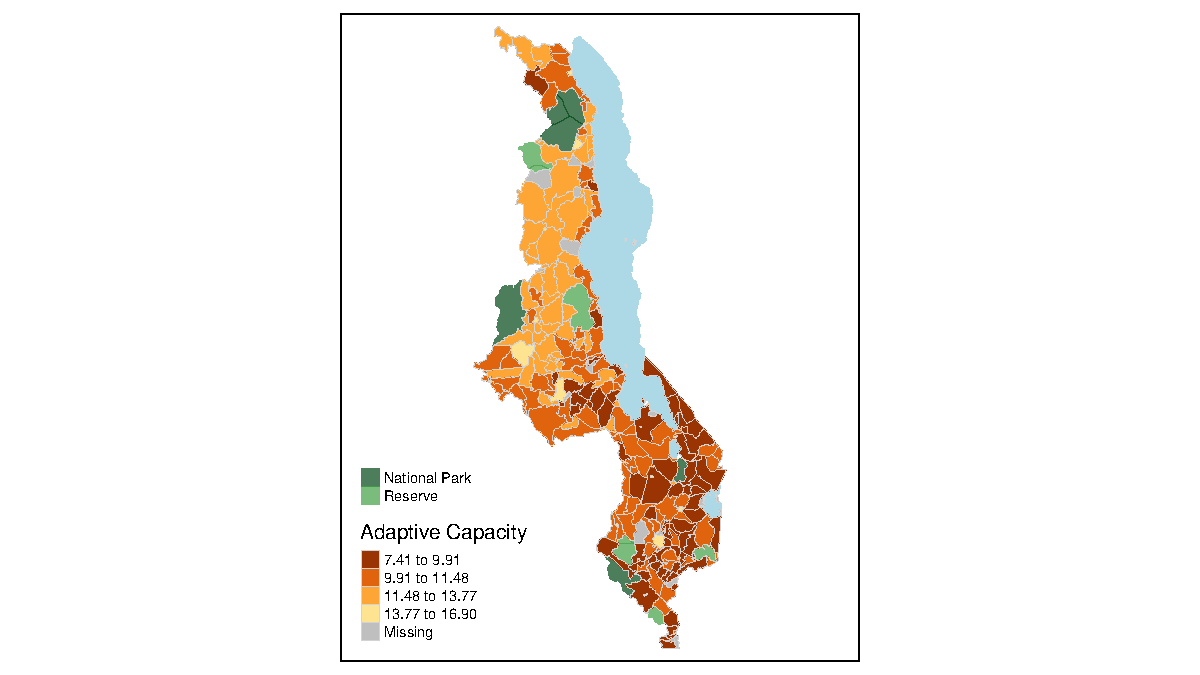
\includegraphics{C:/Users/bcordola/Documents/GitHub/RPr-Malcomb-2014/results/figures/reproduction-figure-4-map-1.pdf}

\hypertarget{evaluate-adaptive-capacity-reproduction}{%
\subsubsection{Evaluate adaptive capacity
reproduction}\label{evaluate-adaptive-capacity-reproduction}}

In order to test the adaptive capacity results, we will georeference the
original figure 4 map using the QGIS3 georeferencer plugin. Using a
vector dataset of traditional authorities and the georeferenced map, we
will then use zonal statistics to extract the average brightness values,
(which represent four classes of adaptive capacity) for each traditional
authority. We will use an interior buffer of the traditional authority
polygons, optimized in order to avoid summarizing border symbol in zonal
statistics while capturing as much of the choropleth color symbol as
possible. After inspecting a histogram of the mean brightness values, we
will reclassify the values as closely to the four classes on the
original figure 4 as possible and then manually adjust the attribute
values for any misclassified traditional authorities. We will compare
original and reproduction household resilience results by creating a
confusion matrix, calculating the Spearman's Rho correlation coefficient
(expecting a value of 1 for perfect positive correlation), and creating
a thematic map of the difference between the original results and
replication results.

\hypertarget{digitize-original-study-figure-4}{%
\paragraph{Digitize original study figure
4}\label{digitize-original-study-figure-4}}

Ordinal data from figure 4 was digitized in QGIS with the following
procedure:

\begin{enumerate}
\def\labelenumi{\arabic{enumi}.}
\tightlist
\item
  Copy image from the original publication \texttt{pdf} file using Adobe
  Acrobat Pro
\item
  Paste the image and save as a \texttt{.png} file with pixel dimensions
  1982 by 2811
\item
  Use QGIS 3.26.3 Georeference the map image to match
  \texttt{ta\_v.gpkg} using WGS 84 geographic coordinates (epsg:4326).
  Use linear georeferencing with points in
  \texttt{metadata\textbackslash{}malcomb\_fig4.png.points}
\item
  Make internal buffer to reduce the noise from boundary line symbology.

  \begin{enumerate}
  \def\labelenumii{\arabic{enumii}.}
  \tightlist
  \item
    Project \texttt{ta\_v} to UTM 36S epsg:32736:
    \texttt{ta\_v\_fig4.gpkg:utm36s}.
  \item
    Calculate an internal buffer of \texttt{-600m}:
    \texttt{ta\_v\_fig4.gpkg:utm36s}.
  \item
    Project back to WGS 84 epsg:4326:
    \texttt{ta\_v\_fig4.gpkg:buffer\_wgs84}.
  \end{enumerate}
\item
  Extract the average and standard deviation of the original map's red,
  green, and blue bands for each traditional authority using the zonal
  statistics algorithm: \texttt{ta\_v\_fig4.gpkg:r},
  \texttt{ta\_v\_fig4.gpkg:rb} and \texttt{ta\_v\_fig4.gpkg:rbg}
\item
  Join the zonal statistics results to the \texttt{ta\_v} layer by the
  \texttt{ID\_2} attribute: \texttt{ta\_v\_fig4.gpkg:ta\_v\_fig4}
\item
  Classify the results in a new field \texttt{orac} (original adaptive
  capacity) using the field calculator and \texttt{CASE} statements,
  choosing break points that classify most traditional authorities
  correctly.
\item
  Visually inspect results and edit the \texttt{orac} attribute for any
  mis-classified area.
\item
  The original map contains data in six conservation areas, noted with
  digitized point features in \texttt{ta\_v\_fig4.gpkg:fig4\_errors}.
  Other areas are coded as follows:
\end{enumerate}

\begin{longtable}[]{@{}cc@{}}
\toprule\noalign{}
code & description \\
\midrule\noalign{}
\endhead
\bottomrule\noalign{}
\endlastfoot
-3 & polygon too small to discern color or pattern fill \\
-2 & white fill not matching any legend item \\
-1 & pattern fill for ``missing DHS data'' \\
1 & lowest adaptive capacity \\
2 & \ldots{} \\
3 & \ldots{} \\
4 & highest adaptive capacity \\
\end{longtable}

\hypertarget{original-study-figure-4}{%
\paragraph{Original study figure 4}\label{original-study-figure-4}}

Load digitized figure 4 data and display counts of results. Convert all
forms of missing data to \texttt{NA} to be excluded from mapping and
statistics. Join original figure 4 adaptive capacity results to
\texttt{ta\_v}.

\begin{longtable}[]{@{}rr@{}}
\toprule\noalign{}
orac & n \\
\midrule\noalign{}
\endhead
\bottomrule\noalign{}
\endlastfoot
-3 & 3 \\
-2 & 30 \\
-1 & 3 \\
1 & 38 \\
2 & 56 \\
3 & 72 \\
4 & 37 \\
\end{longtable}

Map original figure 4.

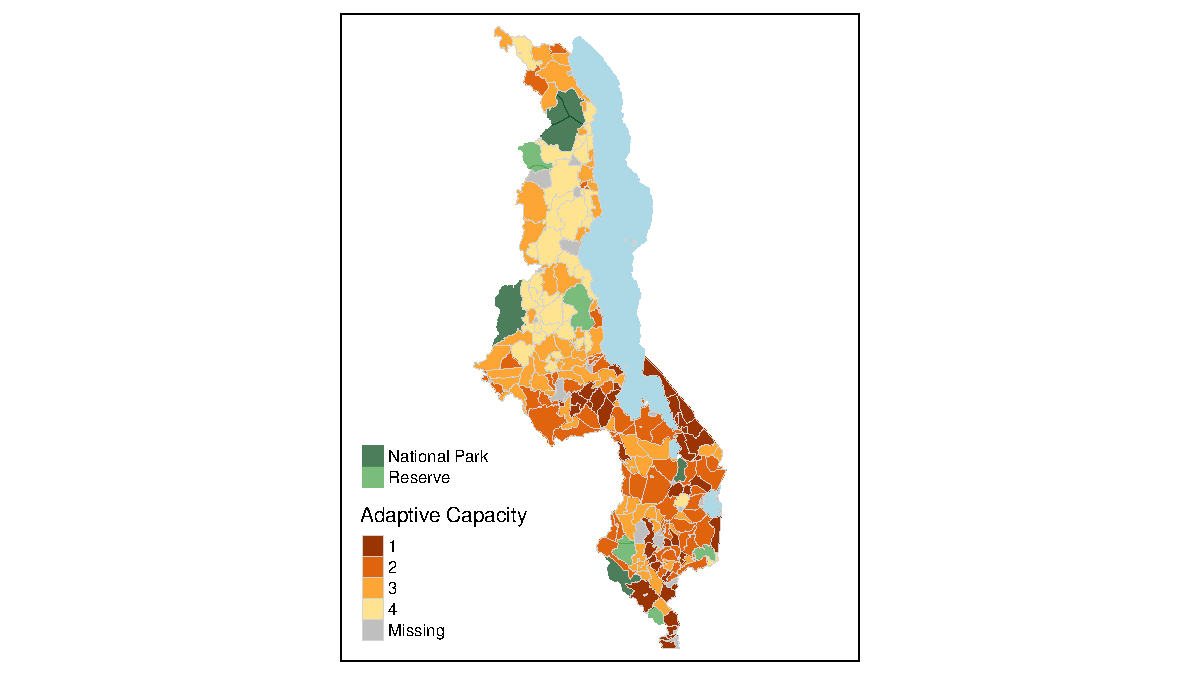
\includegraphics{C:/Users/bcordola/Documents/GitHub/RPr-Malcomb-2014/results/figures/map-original-fig4-1.pdf}

\hypertarget{compare-adaptive-capacity-result}{%
\paragraph{Compare adaptive capacity
result}\label{compare-adaptive-capacity-result}}

Calculate and map difference between the two maps.

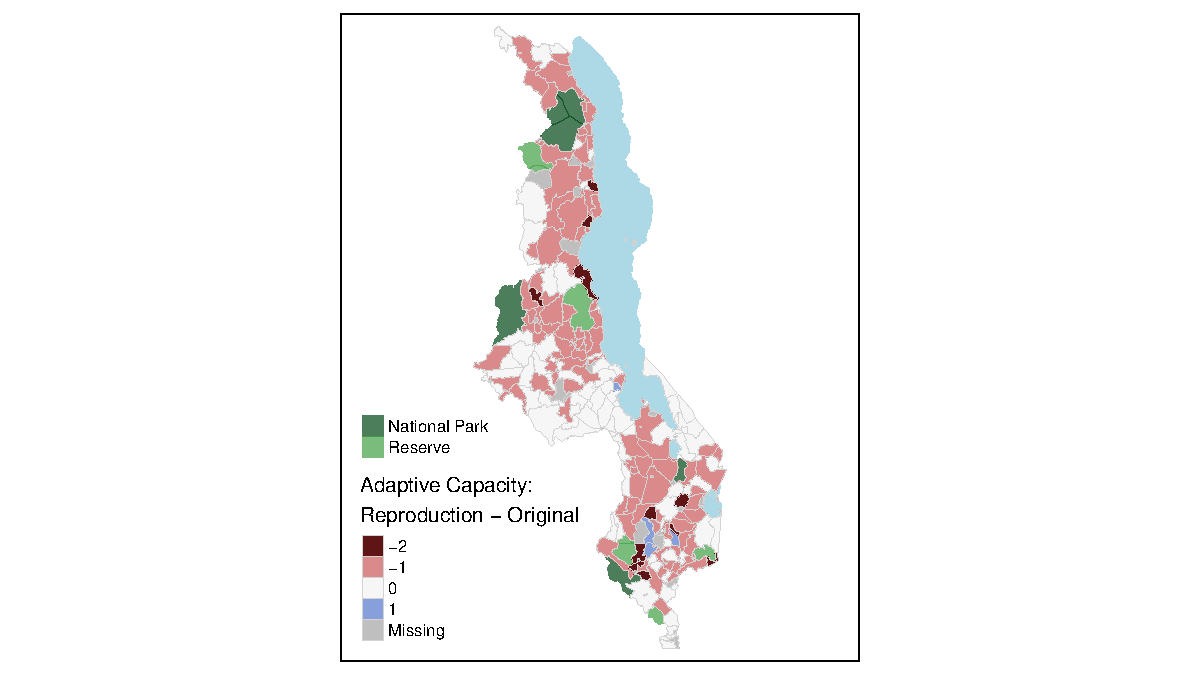
\includegraphics{C:/Users/bcordola/Documents/GitHub/RPr-Malcomb-2014/results/figures/fig4-difference-map-1.pdf}

\begin{verbatim}
##    
##      1  2  3  4
##   1 34 27  6  0
##   2  4 26 44  5
##   3  0  0 19 29
##   4  0  0  0  3
\end{verbatim}

\begin{verbatim}
## 
##  Spearman's rank correlation rho
## 
## data:  ta_v$rpac_class and ta_v$orac
## S = 268637, p-value < 2.2e-16
## alternative hypothesis: true rho is greater than 0
## sample estimates:
##       rho 
## 0.7891711
\end{verbatim}

\hypertarget{vulnerability}{%
\subsection{Vulnerability}\label{vulnerability}}

\begin{itemize}
\tightlist
\item
  40\%: Adaptive Capacity
\item
  20\%: Livelihood Sensitivity (T2)

  \begin{itemize}
  \tightlist
  \item
    ``sensitivity'' defined as ``degree to which a system will respond
    to an external disturbing force'' (2.2) and referred to as:

    \begin{itemize}
    \tightlist
    \item
      ``livelihood sensitivity'' (1.4, 3.3, 3.6, T1 theory, 4.6 formula,
      F5)
    \end{itemize}
  \item
    measured as a positive condition (4.6)
  \end{itemize}
\item
  40\%: Physical exposure (T2)

  \begin{itemize}
  \tightlist
  \item
    ``exposure'' defined as the ``magnitude and frequency of forces that
    could stress a system'' (2.2) and referred to as:

    \begin{itemize}
    \tightlist
    \item
      ``physical exposure'' (1.4, 3.3, 3.7, 4.6 formula, T2)
    \item
      ``biophysical exposure'' (T1 theory)
    \item
      ``exposure to floods and droughts'' (F5)
    \end{itemize}
  \item
    measured as a negative condition (4.6)
  \end{itemize}
\item
  100\%: Household Resilience (T2)

  \begin{itemize}
  \tightlist
  \item
    ``resilience'' defined as ``ability of a household to prepare for,
    respond to and recover from complex drivers of vulnerability'' (2.2,
    5.6) and referred to as:

    \begin{itemize}
    \tightlist
    \item
      ``household resilience'' calculated as ``Adaptive Capacity +
      Livelihood Sensitivity - Physical Exposure'' (4.6 formula)
    \item
      ``vulnerability to climate change'' calculated as ``assets +
      access + livelihood sensitivity - physical exposure'' (F5)
    \item
      ``vulnerability'' (title, 3.3, 3.6, 4.3, 4.5, 6.5, 7.1, 7.2)
    \end{itemize}
  \end{itemize}
\end{itemize}

\hypertarget{extent-and-spatial-resolution}{%
\subsubsection{Extent and spatial
resolution}\label{extent-and-spatial-resolution}}

Create bounding box representing the spatial extent of Malawi. Create a
raster grid frame matching the extent of the bounding box and the
spatial resolution of the drought exposure raster, which is
\texttt{0.041667} decimal degrees. Although the flood risk raster has a
coarser spatial resolution, visual inspection of the original figure 5
suggests that the finer spatial resolution of drought exposure was used
for the original analysis.

\hypertarget{adaptive-capacity-1}{%
\subsubsection{Adaptive capacity}\label{adaptive-capacity-1}}

Convert adaptive capacity to raster grid.

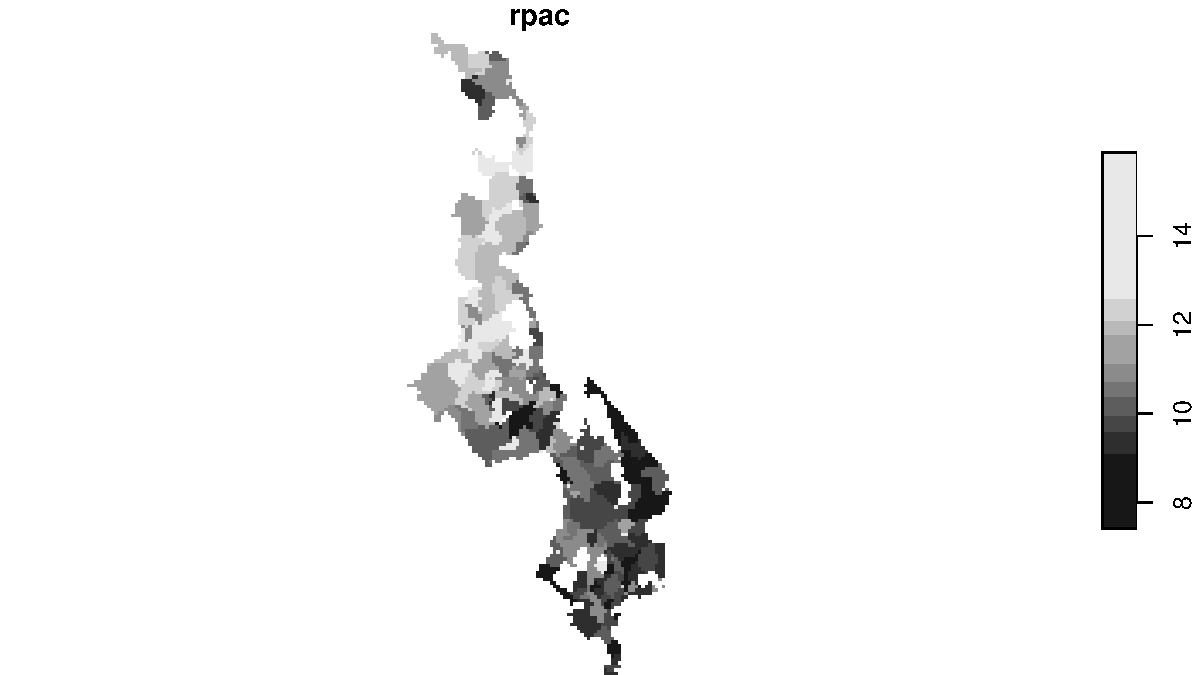
\includegraphics{C:/Users/bcordola/Documents/GitHub/RPr-Malcomb-2014/results/figures/rasterizing-geometries-1.pdf}

\hypertarget{drought-exposure}{%
\subsubsection{Drought exposure}\label{drought-exposure}}

Clip and warp drought exposure to match our extent and spatial
resolution.

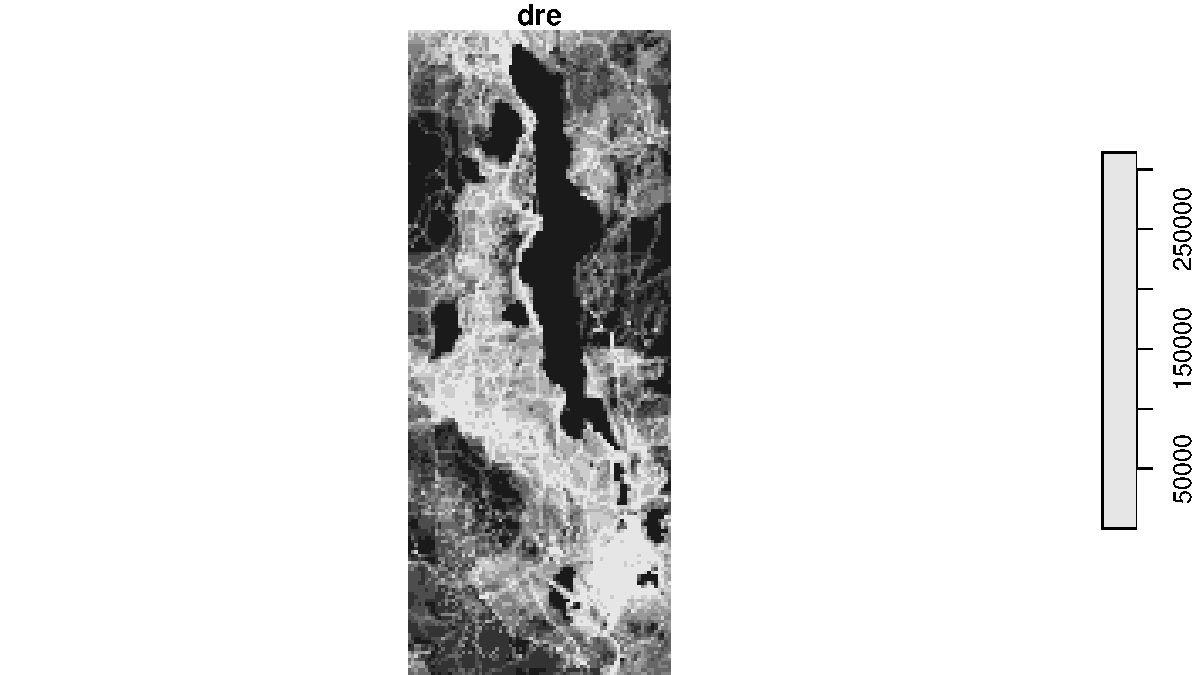
\includegraphics{C:/Users/bcordola/Documents/GitHub/RPr-Malcomb-2014/results/figures/clip-map-drought-exposure-1-1.pdf}
Create a mask with the adaptive capacity results so that lakes,
conservation areas, and traditional authorities with no data will not
skew the classification / rescaling of drought exposure. Apply this mask
to drought exposure. Masking is our own decision based on intuition: it
is not specified in the original publication.

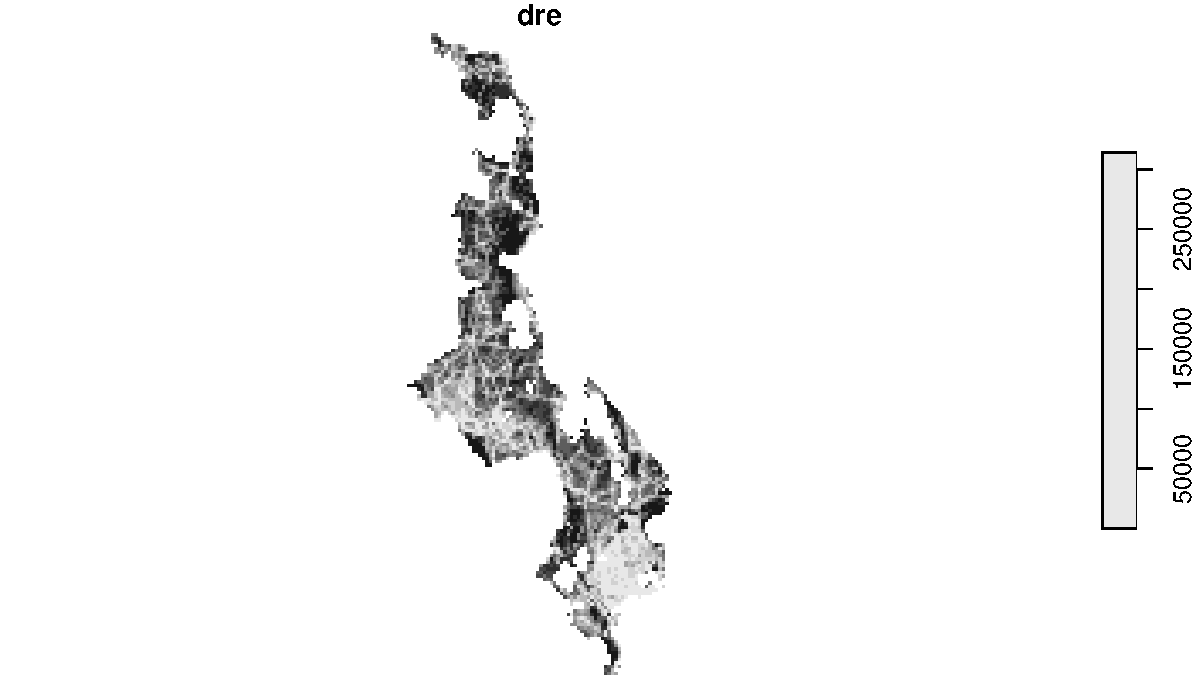
\includegraphics{C:/Users/bcordola/Documents/GitHub/RPr-Malcomb-2014/results/figures/create-mask-1.pdf}

Classify drought exposure into quintile classes (0 to 4) Then rescale to
20\% by multiplying by 5.

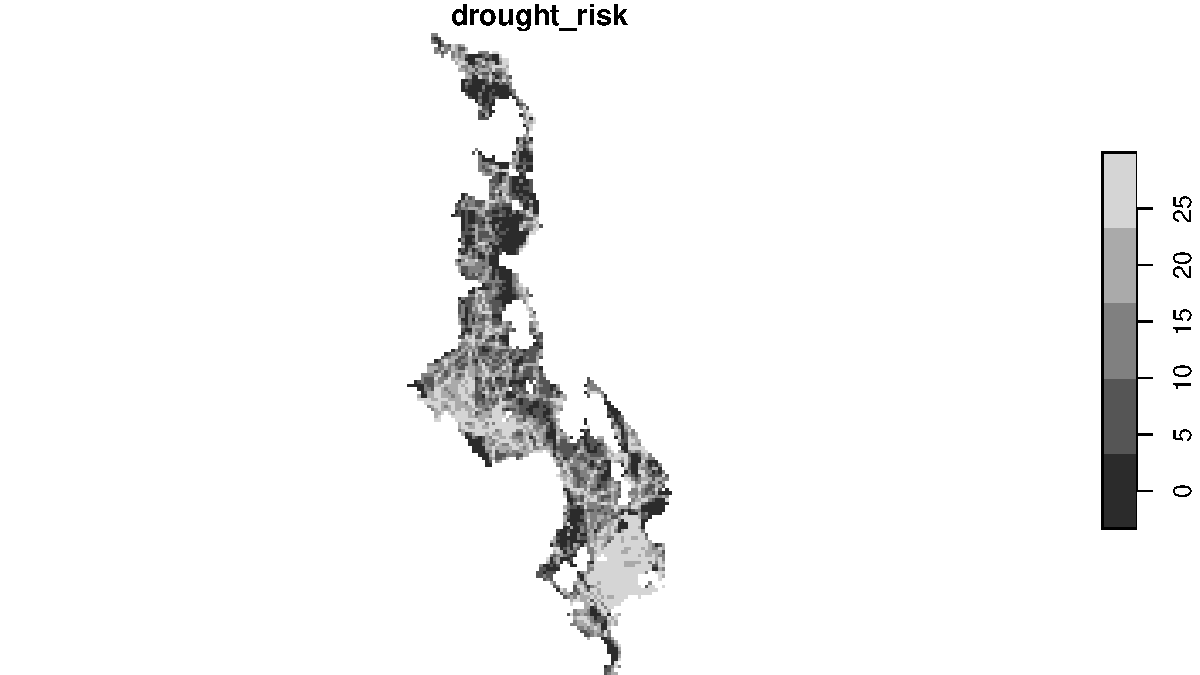
\includegraphics{C:/Users/bcordola/Documents/GitHub/RPr-Malcomb-2014/results/figures/drought-rescale-1.pdf}

\hypertarget{flood-risk}{%
\subsubsection{Flood risk}\label{flood-risk}}

Clip and warp flood risk to match our extent and spatial resolution.

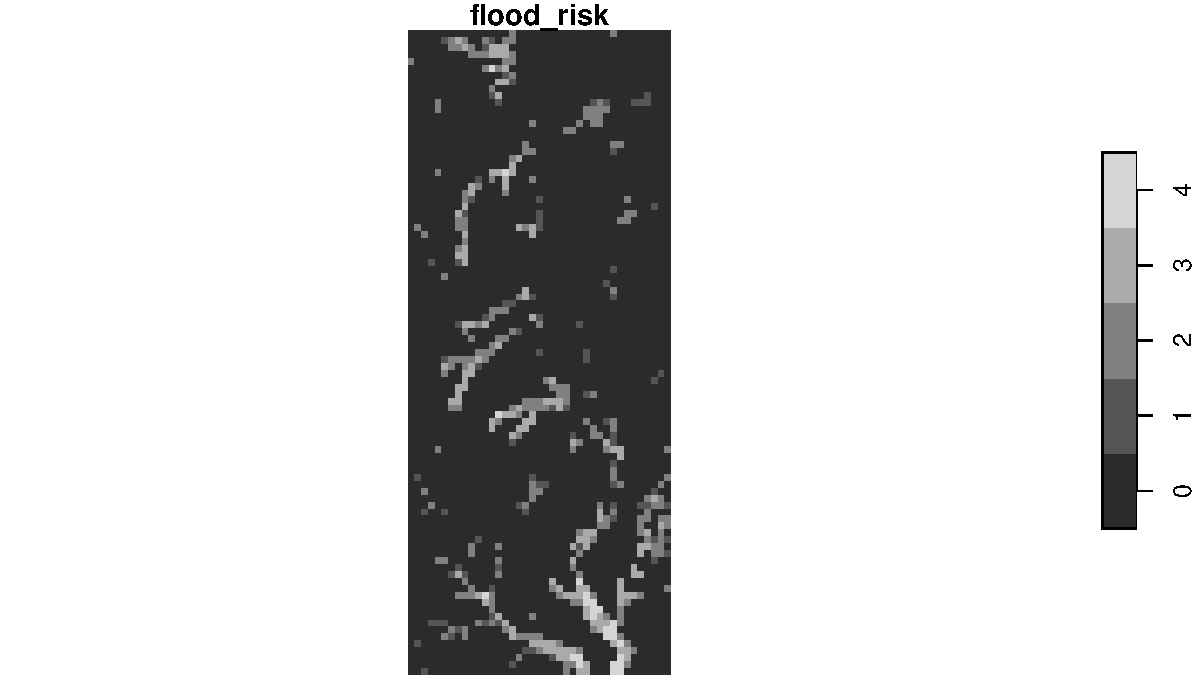
\includegraphics{C:/Users/bcordola/Documents/GitHub/RPr-Malcomb-2014/results/figures/clip-map-drought-exposure-2-1.pdf}
Mask and rescale flood. \#\# My CHANGE - MULTIPLY BY 3.333 INSTEAD OF 5
\#\#\# Since flood is already on scale from 0 to 4, simply multiply by
3.333 to achieve the 20\% weight.

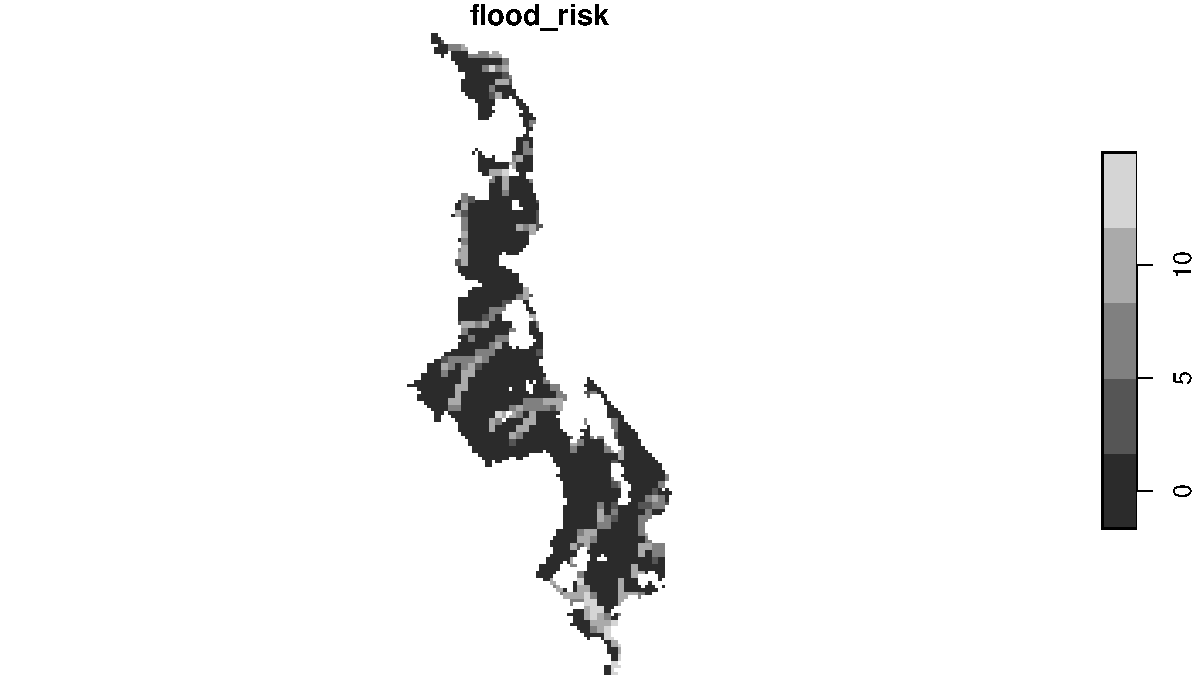
\includegraphics{C:/Users/bcordola/Documents/GitHub/RPr-Malcomb-2014/results/figures/mask-and-rescale-flood-1.pdf}

\hypertarget{livelihood-sensitivity}{%
\subsubsection{Livelihood sensitivity}\label{livelihood-sensitivity}}

Calculate livelihood sensitivity indicators from FEWSnet livelihood zone
baseline profiles of poor households according to table 2.

Rescale livelihood sensitivity indicators into quantiles.

\begin{verbatim}
##              pctOwnCrop pctIncWage pctIncCashCrops pctDisasterCope ownCrop
## nbr.val            18.0       18.0            18.0            18.0    18.0
## nbr.null            0.0        0.0            13.0             1.0     1.0
## nbr.na              0.0        0.0             0.0             0.0     0.0
## min                29.4        9.7             0.0             0.0     0.0
## max                88.0       50.3            75.1            71.9     4.0
## range              58.6       40.6            75.1            71.9     4.0
## sum              1059.3      489.6           171.8           236.5    36.0
## median             55.0       24.7             0.0             8.8     2.0
## mean               58.9       27.2             9.5            13.1     2.0
## SE.mean             3.1        2.6             5.3             3.7     0.3
## CI.mean.0.95        6.6        5.5            11.2             7.9     0.6
## var               176.8      121.3           507.8           251.0     1.6
## std.dev            13.3       11.0            22.5            15.8     1.3
## coef.var            0.2        0.4             2.4             1.2     0.6
##              wageIncome cashCropIncome disasterCope
## nbr.val            18.0           18.0         18.0
## nbr.null            1.0            1.0          1.0
## nbr.na              0.0            0.0          0.0
## min                 0.0            0.0          0.0
## max                 4.0            1.2          4.0
## range               4.0            1.2          4.0
## sum                36.0           17.6         36.0
## median              2.0            1.2          2.0
## mean                2.0            1.0          2.0
## SE.mean             0.3            0.1          0.3
## CI.mean.0.95        0.6            0.2          0.6
## var                 1.6            0.1          1.6
## std.dev             1.3            0.4          1.3
## coef.var            0.6            0.4          0.6
\end{verbatim}

Calculate aggregate livelihood sensitivity score

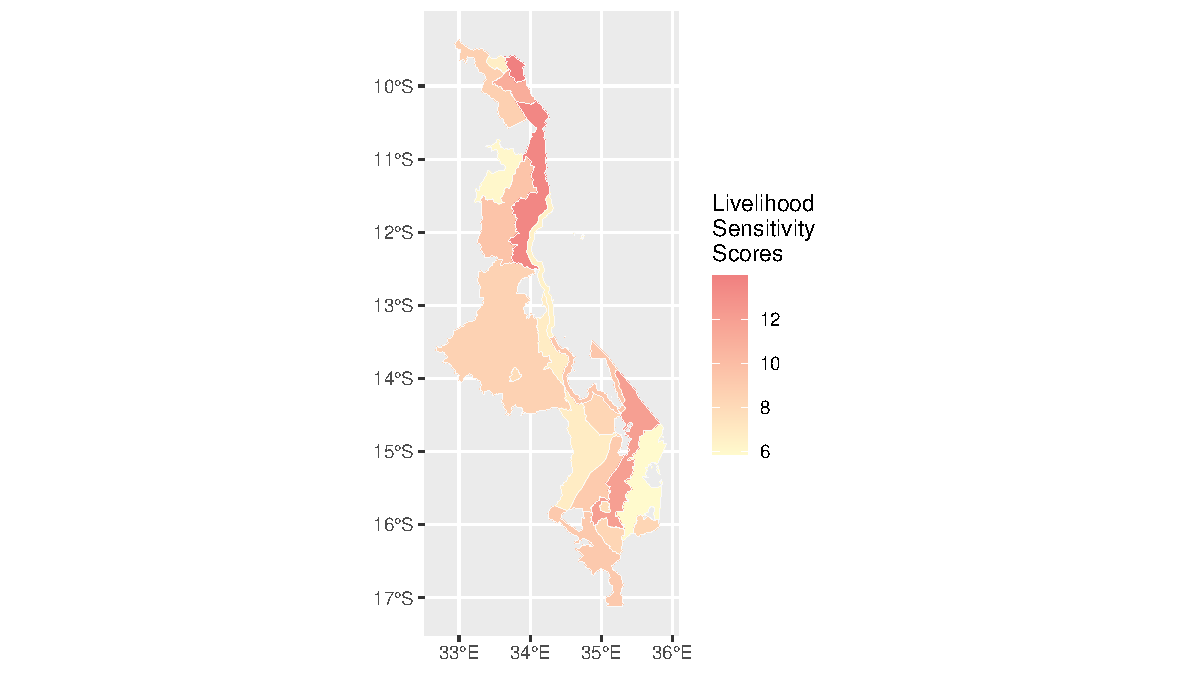
\includegraphics{C:/Users/bcordola/Documents/GitHub/RPr-Malcomb-2014/results/figures/calculate-livelihood-sensitivity-1.pdf}

\begin{verbatim}
##              sensitivity
## nbr.val            18.00
## nbr.null            0.00
## nbr.na              0.00
## min                 5.88
## max                14.00
## range               8.12
## sum               161.65
## median              8.65
## mean                8.98
## SE.mean             0.56
## CI.mean.0.95        1.18
## var                 5.65
## std.dev             2.38
## coef.var            0.26
\end{verbatim}

Convert livelihood sensitivity into raster grid

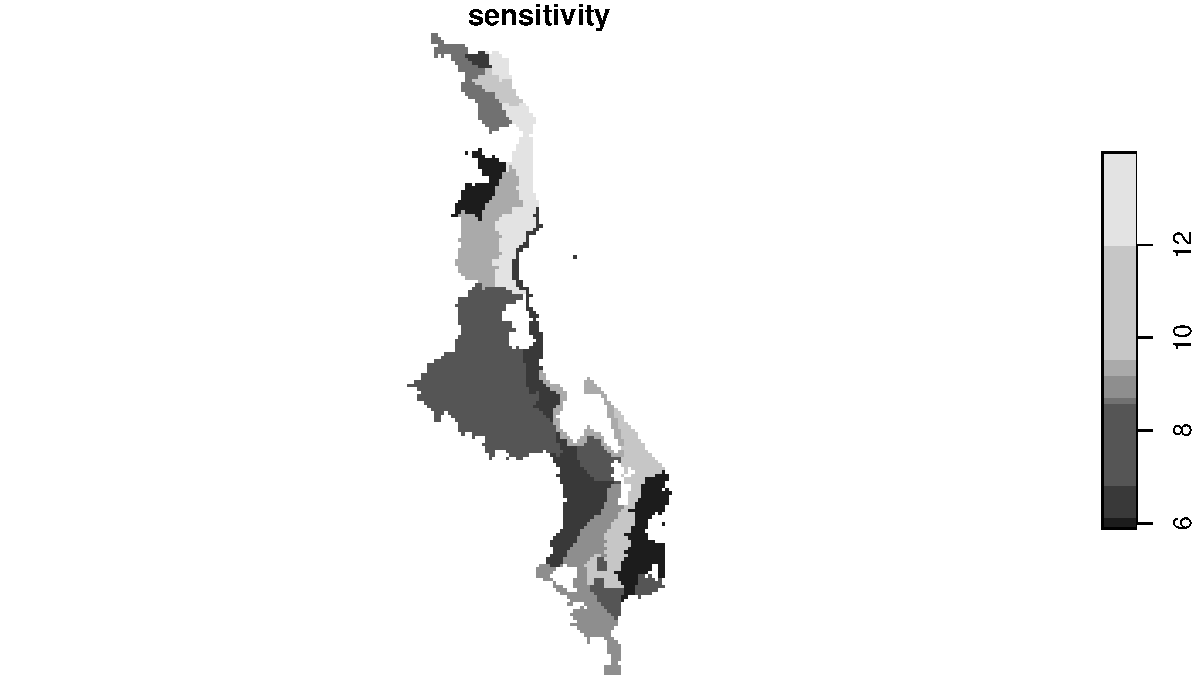
\includegraphics{C:/Users/bcordola/Documents/GitHub/RPr-Malcomb-2014/results/figures/sensitivity-raster-1.pdf}

\hypertarget{vulnerability-score}{%
\subsubsection{Vulnerability score}\label{vulnerability-score}}

Calculate an aggregated vulnerability score by adding low adaptive
capacity (invert adaptive capacity by subtracting from the maximum score
of 40), livelihood sensitivity, drought exposure, and flood risk.

\[
Vulnerability = (40 - Adaptive Capacity) + Livelihood Sensitivity + Drought Exposure + Flood Risk
\]

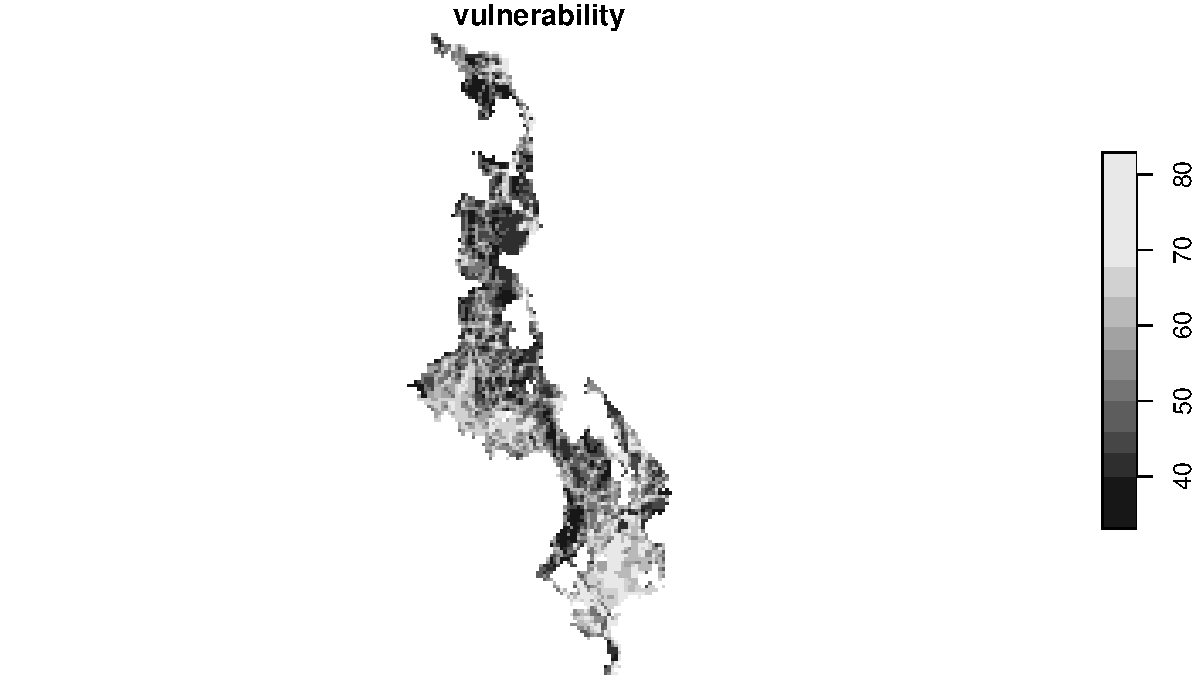
\includegraphics{C:/Users/bcordola/Documents/GitHub/RPr-Malcomb-2014/results/figures/combined-vulnerability-1.pdf}

\hypertarget{reproduction-figure-5}{%
\subsubsection{Reproduction figure 5}\label{reproduction-figure-5}}

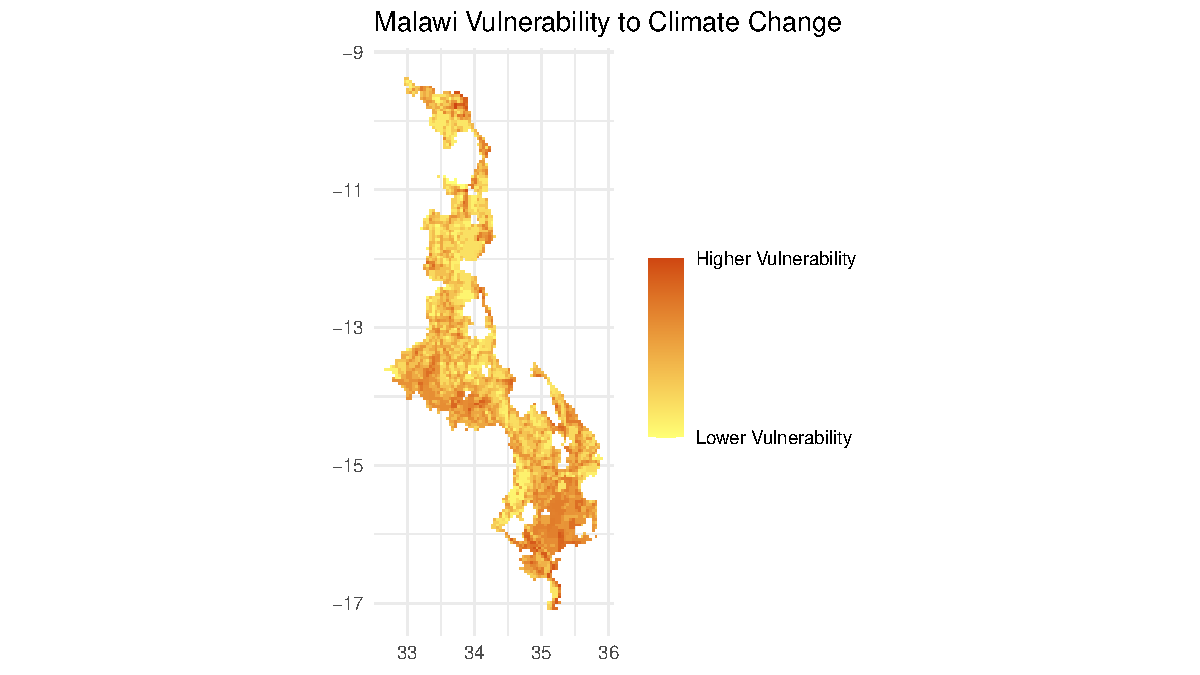
\includegraphics{C:/Users/bcordola/Documents/GitHub/RPr-Malcomb-2014/results/figures/vulnerability-map-1.pdf}

\hypertarget{evaluate-vulnerability-reproduction}{%
\subsubsection{Evaluate vulnerability
reproduction}\label{evaluate-vulnerability-reproduction}}

In order to compare the Malawi vulnerability results, we will
georeference the original figure 5 map using QGIS georeferencer plugin.
We will vectorize the UNEP-Grid raster input most closely matching the
published map and summarize the red, green, and blue brightness values
of the original map using zonal statistics. We will add the green and
blue brightness values together to convert the original color ramp into
a linear scale of continuous values. We will compare original and
reproduction Malawi vulnerability results by creating a scatterplot,
Spearman's Rho correlation coefficient (expecting a value near 1 for
perfect positive correlation), and thematic map of the difference
between the original results and replication results.

\hypertarget{original-study-figure-5}{%
\paragraph{Original study figure 5}\label{original-study-figure-5}}

Comparing the reproduction of figure 5 with the original figure 5
requires first digitizing the original figure 5 (unclassified choropleth
map with yellow to red gradient) in QGIS as follows:

\begin{enumerate}
\def\labelenumi{\arabic{enumi}.}
\tightlist
\item
  Copy image of figure 5 from the original publication \texttt{pdf} file
  using Adobe Acrobat Pro
\item
  Paste the image and save as a \texttt{.png} file with pixel dimensions
  1949 by 2811
\item
  Use QGIS 3.26.3 Georeference the map image to match
  \texttt{ta\_v.gpkg} using WGS 84 geographic coordinates (epsg:4326).
  Use linear georeferencing with points in \texttt{...}
\item
  Convert \texttt{ta\_capacity.tif} raster to vector polygons
\item
  Extract the average blue and green bands from the georeferenced map
  image using \texttt{zonal\ statistics}
\item
  Save results as \texttt{georef\_bg.gpkg}.
\end{enumerate}

To approximate data values from the yellow to red gradient of the
original map, the blue and green bands are then added, inverted, and
rescaled to a range from 0 to 100.

\hypertarget{compare-vulnerability-result}{%
\paragraph{Compare vulnerability
result}\label{compare-vulnerability-result}}

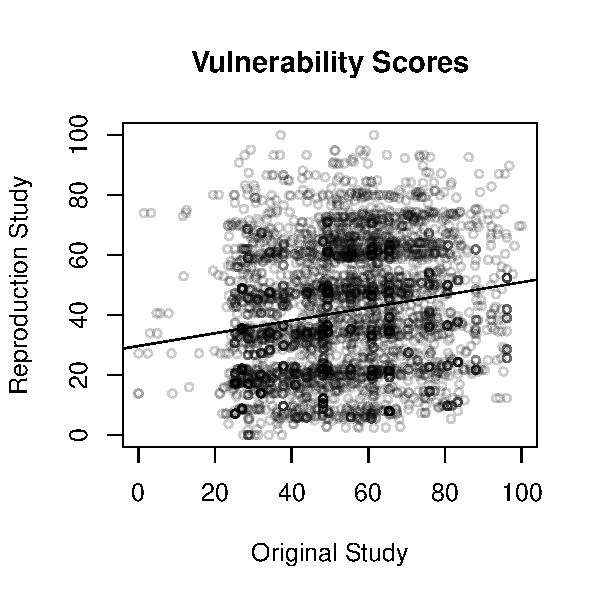
\includegraphics{C:/Users/bcordola/Documents/GitHub/RPr-Malcomb-2014/results/figures/compare-fig5-1.pdf}

\begin{verbatim}
## 
##  Spearman's rank correlation rho
## 
## data:  vulnerability_p$orv and vulnerability_p$rpv
## S = 7058278811, p-value < 2.2e-16
## alternative hypothesis: true rho is not equal to 0
## sample estimates:
##       rho 
## 0.2007671
\end{verbatim}

Map differences in Figure 5

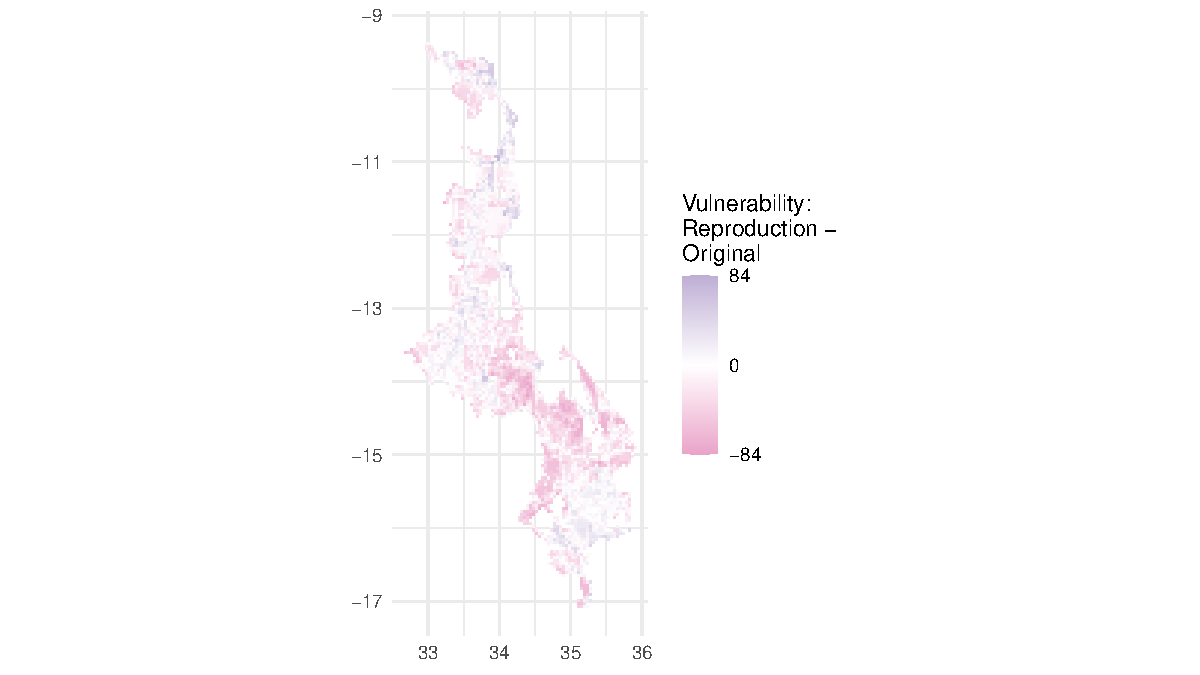
\includegraphics{C:/Users/bcordola/Documents/GitHub/RPr-Malcomb-2014/results/figures/vulnerability-difference-map-1.pdf}

\hypertarget{discussion}{%
\section{Discussion}\label{discussion}}

\hypertarget{conclusions}{%
\section{Conclusions}\label{conclusions}}

\hypertarget{integrity-statement}{%
\section{Integrity Statement}\label{integrity-statement}}

This report and its preregistration were written after already
attempting the reproduction study, including acquisition and analysis of
all of the secondary data sources required. However, the preregistered
analysis plan was written \emph{as if} we had no prior knowledge of the
data other than what is documented in the study. Holler has previously
reviewed and compared other climate vulnerability models for Malawi, and
conducted a scoping study in the Lilongwe and Mangochi districts of
Malawi in 2015, including meeting with the Regional Centre for Mapping
of Resources for Development (RCMRD) consultants who created the Malawi
Hazards and Vulnerability Atlas
(\href{https://doi.org/10.13140/RG.2.1.1460.0402}{2015}).

\hypertarget{references}{%
\section{References}\label{references}}

\hypertarget{referencing-the-original-paper}{%
\subsection{Referencing the original
paper}\label{referencing-the-original-paper}}

Malcomb, D. W., E. A. Weaver, and A. R. Krakowka. 2014. Vulnerability
modeling for sub-Saharan Africa: An operationalized approach in Malawi.
\emph{Applied Geography} 48:17--30.
\url{DOI:\%5B10.1016/j.apgeog.2014.01.004}{]}(\url{https://doi.org/10.1016/j.apgeog.2014.01.004}).

\hypertarget{sections}{%
\subsubsection{Sections}\label{sections}}

\begin{enumerate}
\def\labelenumi{\arabic{enumi}.}
\tightlist
\item
  Introduction
\item
  Complex vulnerability
\item
  Evidence-based Indicators
\item
  Methodology
\item
  Results
\item
  Discussion
\item
  Conclusion
\end{enumerate}

\hypertarget{tables-figures-other-elements}{%
\subsubsection{Tables, figures, other
elements}\label{tables-figures-other-elements}}

\begin{itemize}
\tightlist
\item
  T1 Evidence-based complex vulnerability indicators
\item
  T2 Weighted indicators by metatheme
\item
  F1 Map of Malawi
\item
  F2 Vulnerability web
\item
  F3 Malawi Household Resilience (2004)
\item
  F4 Malawi Household Resilience (2010)
\item
  F5 Malawi Composite Vulnerability Index
\item
  A1 Appendix 1
\item
  R References
\end{itemize}

\hypertarget{other-references}{%
\subsection{Other References}\label{other-references}}

Barrett, S. 2014. Subnational Climate Justice? Adaptation Finance
Distribution and Climate Vulnerability. World Development 58:130--142.
DOI:
\href{http://dx.doi.org/10.1016/j.worlddev.2014.01.014}{10.1016/j.worlddev.2014.01.014}.
Gallopín, G. C. 2006. Linkages Between Vulnerability, Resilience, and
Adaptive Capacity. Global Environmental Change 16 (3):293--303. DOI:
\href{https://doi.org/10.1016/j.gloenvcha.2006.02.004}{10.1016/j.gloenvcha.2006.02.004}.
Rufat, S., E. Tate, C. G. Burton, and A. S. Maroof. 2015. Social
vulnerability to floods: Review of case studies and implications for
measurement. \emph{International Journal of Disaster Risk Reduction}
14:470--486. DOI:
\href{http://dx.doi.org/10.1016/j.ijdrr.2015.09.013}{10.1016/j.ijdrr.2015.09.013}.
Smit, B., and J. Wandel. 2006. Adaptation, adaptive capacity and
vulnerability. Global Environmental Change 16 (3):282--292. DOI:
\href{https://doi.org/10.1016/j.gloenvcha.2006.03.008}{10.1016/j.gloenvcha.2006.03.008}.

\end{document}
